\begin{definition}
    Оператор $A: L_2[a, b] \to L_2[a, b]$ называется оператором Гильберта--Шмидта, если 
    \[ (Af)(x) = \int_a^b K(x,t) f(t) dt, \quad K \in L_2([a,b]^2) \]
\end{definition}

\begin{theorem}
    Оператор Гильберта--Шмидта является компактным
\end{theorem}

\begin{proof}
    Хотим воспользоваться теоремой \nameref{12.1}: взять последовательность конечномерных операторов $A_n$, которая сходится по операторной норме к $A$

    $H$~--- сепарабельно, $\{ e_n \}$~--- ОНБ. Тогда $H \ni x = \sum (x, e_n) e_n$

    \begin{theorem}[книжка Колмогорова-Фомина; гл. VII, пар.3, п.5]
        Если $\{ \varphi_n \}$~--- ОНБ в $L_2[a,b]$, то $\{ \varphi_i(x)\varphi_j(t) \}$~--- ОНБ в $L_2([a,b]^2)$
        % идея: аннулятор
    \end{theorem}

    \begin{unnecessary}
    \begin{proof}
    \begin{figure}[H]
    \centering
    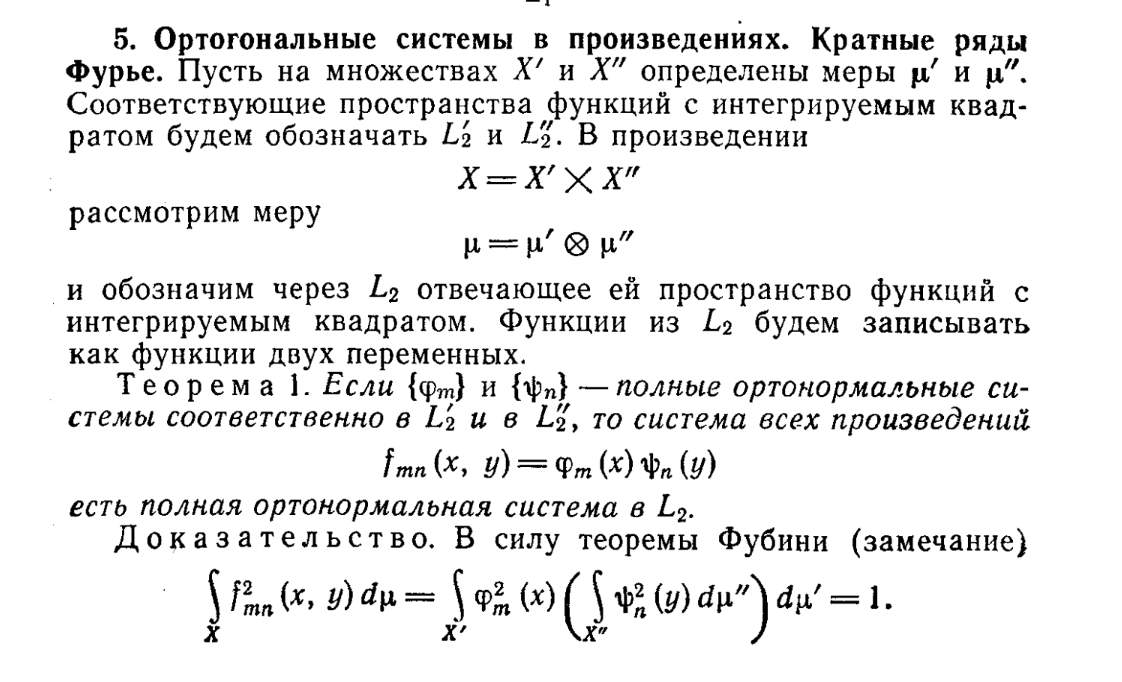
\includegraphics[width=0.6\textwidth]{images/8_2_1.png}\\
    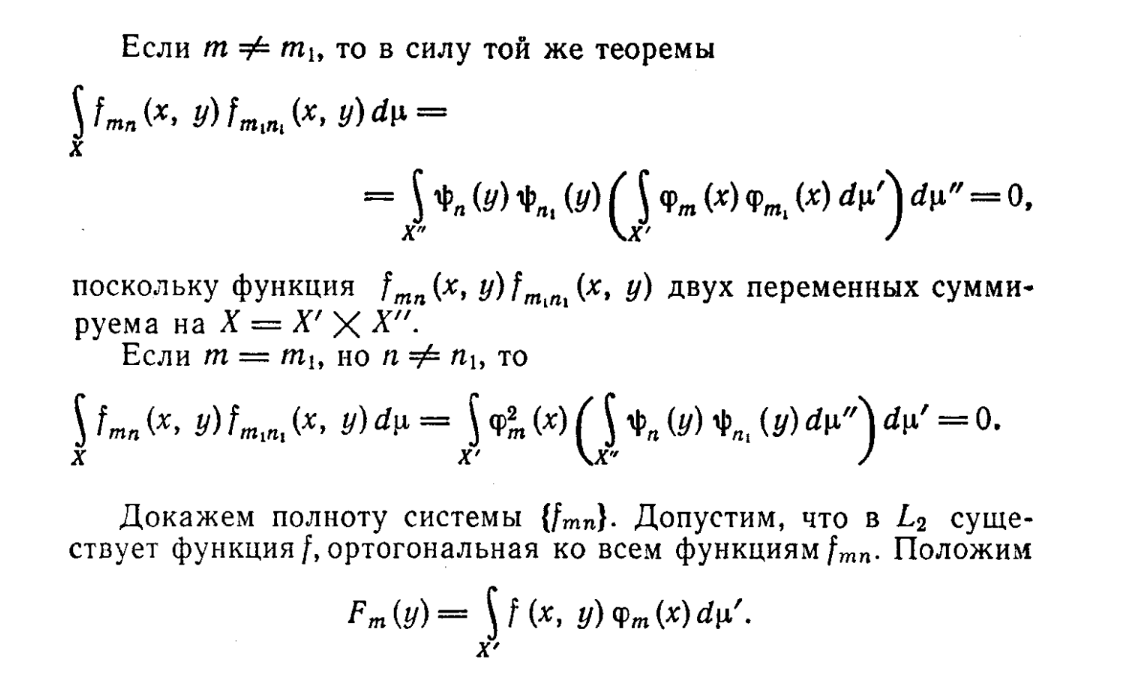
\includegraphics[width=0.6\textwidth]{images/8_2_2.png}\\
    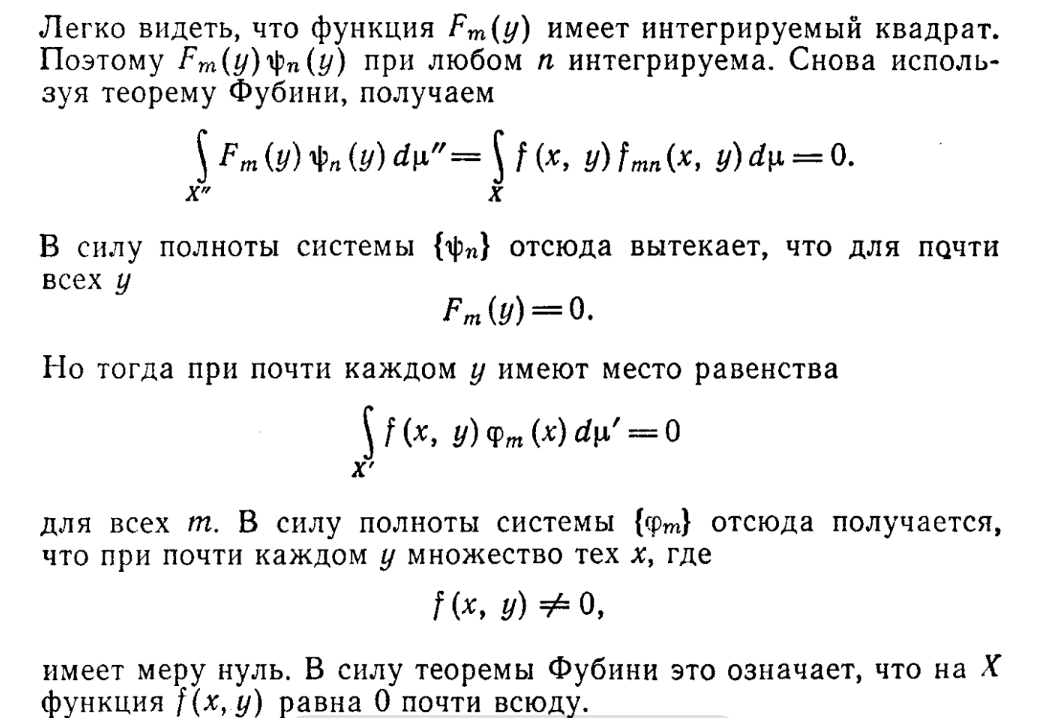
\includegraphics[width=0.6\textwidth]{images/8_2_3.png}\\
    \end{figure}
    \end{proof}
    \end{unnecessary}
    
    Пока примем теорему как верную и будем пользоваться ей. Пусть $\{ \varphi_n \}$~--- ОНБ в $L_2[a,b]$, тогда по теореме $\{ \varphi_i(x) \varphi_j(t) \}$~--- ОНБ в $L_2([a,b]^2)$. Разложим $K$ в ряд Фурье

    \[ K(x,t) = \sum_{i,j} a_{ij} \varphi_i(x) \varphi_j(t) \]

    Возьмем частичные суммы

    \[ K_N(x,t) = \sum_{i,j=1}^N a_{ij} \varphi_i(x) \varphi_j(t) \]

    С каждым ядром свяжем последовательность операторов $A_N$. 
    Два вопроса
    \begin{enumerate}
        \item $A_N$~--- конечномерные
        \[ \int \sum_{i,j=1}^n a_{ij} \varphi_i(x) \varphi_j(t) f(t) dt = \sum_{i=1}^n c_i \varphi_i(x)\]
        Очевидно, что это конечномерный оператор
        \item $\| A_N - A \| \to 0$
        $K_N \xrightarrow[]{L_2} K$. 

        Заметим, что $\|K_n - K\|_{2} \to 0$, поскольку $K_n$ --- частичные суммы ряда Фурье.

        Далее воспользуемся этим и докажем, что $\|A_n - A\| \to 0$. 

        $A_n - A = \int_a^b (K_n(s, t) - K(s, t))x(t)dt$, которое является скалярным произведением векторов $(K_n - K)_s(t) \text{ и } \overline{x(t)} \text{в} L_2[a,b]$. При этом из неравенства Коши--Буняковского получаем $|A_n - A| \leq \|(K_n - K)_s\|_{2} \|x\|_{2}$. Отсюда с учётом теоремы Фубини получаем 
        $$\int_a^b|(A_n - A)(s)|^2 ds \leq \Big(\int_a^b \|(K_n - K)_s\|_{2}^2 \Big)\|x\|_2^2 = \Big(\int_a^b \int_a^b |(K_n - K)(s,t)|^2dsdt\Big)\|x\|_2^2$$

        Указанный двойной интеграл это $\|K_n - K\|_2^2$, поэтому $(A_n - A) \in L_2[a,b] \text{ и } \|A_n - A\|_2 \leq \|K_n - K\|_2 \cdot \|x\|_2$

        Таким образом, получим нужную сходимость.
    \end{enumerate}
\end{proof}